\section{Additional Discussion for Public Benchmark Evaluation}
\label{ap:disucuss_public}

% \zixuan{TODO: add additional discussion}

\subsection{Sub-agents and Baselines Setup}
\label{ap:discuss_baselines}

For \texttt{SearchAgent}, we adapt the OpenDeepResearch code\footnote{\url{https://github.com/langchain-ai/open_deep_research}}
 to use DuckDuckGo Search\footnote{\url{https://duckduckgo.com/}}
 for HotpotQA and a BM25 retriever \citep{robertson1994okapi} for BrowseComp+. \cref{tab:baseline_setup} summarizes the sub-agents, including the orchestration decisions in \ourframework (i.e, configurations required to be generated by the orchestrator), and their corresponding implementations.

\begin{table*}[h]
\centering
\small
% \addtolength{\tabcolsep}{-0.4em}
\begin{tabular}{l l l}
\toprule
\textbf{Sub-agent} & \textbf{Orchestration Decisions} & \textbf{Implementation} \\
\midrule
CoTAgent & Input & \cref{app:sub_agents} \\
SCAgent & Input & \cref{app:sub_agents} \\
ReflexionAgent & Input & \cref{app:sub_agents} \\
DebateAgent & Input, Debate role & \cref{app:sub_agents} \\
SearchAgent (HotpotQA) & Input & Autonomous (Multi-turn + DuckDuckGoSearch) \\
SearchAgent (BrowseComp+) & Input & Autonomous (Multi-turn + BM25) \\
\bottomrule
\end{tabular}
\caption{Summary of the sub-agents.
}
\label{tab:baseline_setup}
\end{table*}

For baseline systems, we run all baselines using the official code released by the original authors.

\subsection{Additional Observations on Overall Results}
\label{ap:addition_observation}


\cref{sec:experiemnt} reports the superiority of \ourframework over all baselines. In this section, we provide additional observations based on our experience running these systems.

\paragraph{Inference-time orchestration baselines.}
Inference-time orchestration methods are often computationally costly, particularly AFlow and MAS-Zero. MAS-Zero requires an orchestrator larger than 32B parameters to produce meaningful results, as also noted in the original paper \citep{Ke2025MASZero}. AFlow achieves the strongest baseline performance among inference-time methods, but still underperforms \ourframework by a clear margin.

\paragraph{Training-based orchestration baselines.}
Training-based orchestration baselines perform unexpectedly worse than many inference-time methods. We observe that MAS-GPT frequently falls back to Self-Consistency (SC), which itself is a strong single-agent system, when no valid MAS are generated. This fallback behavior contributes substantially to its reported gains when compared with ToolOrchestra.

We further observe that ToolOrchestra often refuses to call any tool. In ToolOrchestra, the sub-agent is treated as a tool, and such refusal results in degraded performance when the sub-agent is stronger than the orchestrator for solving the task. In contrast, \ourframework does not rely on any manually designed fallback strategy. All MAS are generated directly by the learned orchestrator. Under the DoM notation, sub-agents in \ourframework are consistently and effectively utilized, as illustrated in Figures \ref{fig:7b_120b_aime24_low}, \ref{fig:7b_120b_browse_comp_plus_high}, and \ref{fig:7b_120b_hotpotqa_high}.

%TODO??
 % Importantly, on AIME24 and GPQA—which are predominantly sequential tasks (see \cref{sec:experiemnt})—SAS or simple standalone sub-agents can outperform automatic MAS design methods, as these benchmarks do not operate at the edge of sub-agent competence where MAS are most effective.
 
% \zixuan{talk about baselines setting and observations (e.g., toolorchestae ofern time does not call any tool)}

\begin{center}
\vspace{-0.5\baselineskip}
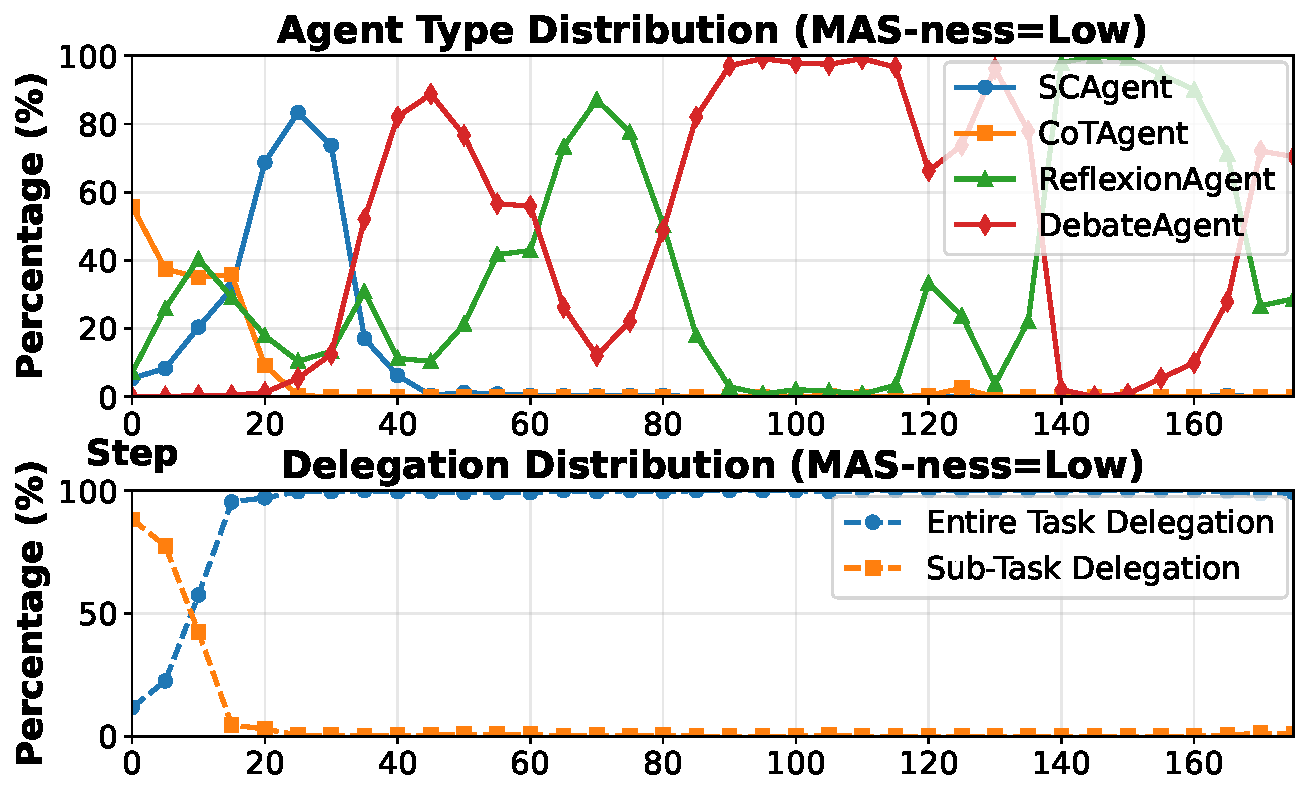
\includegraphics[width=0.5\columnwidth]{figs/7b_120b_aime24_low.pdf}
% \vspace{-1.5\baselineskip}
\captionof{figure}{\small Statistics of agents for low \masness (AIME24).}
\label{fig:7b_120b_aime24_low}
\end{center}


\begin{figure*}[h]
\centering
% \vspace{-2\baselineskip}
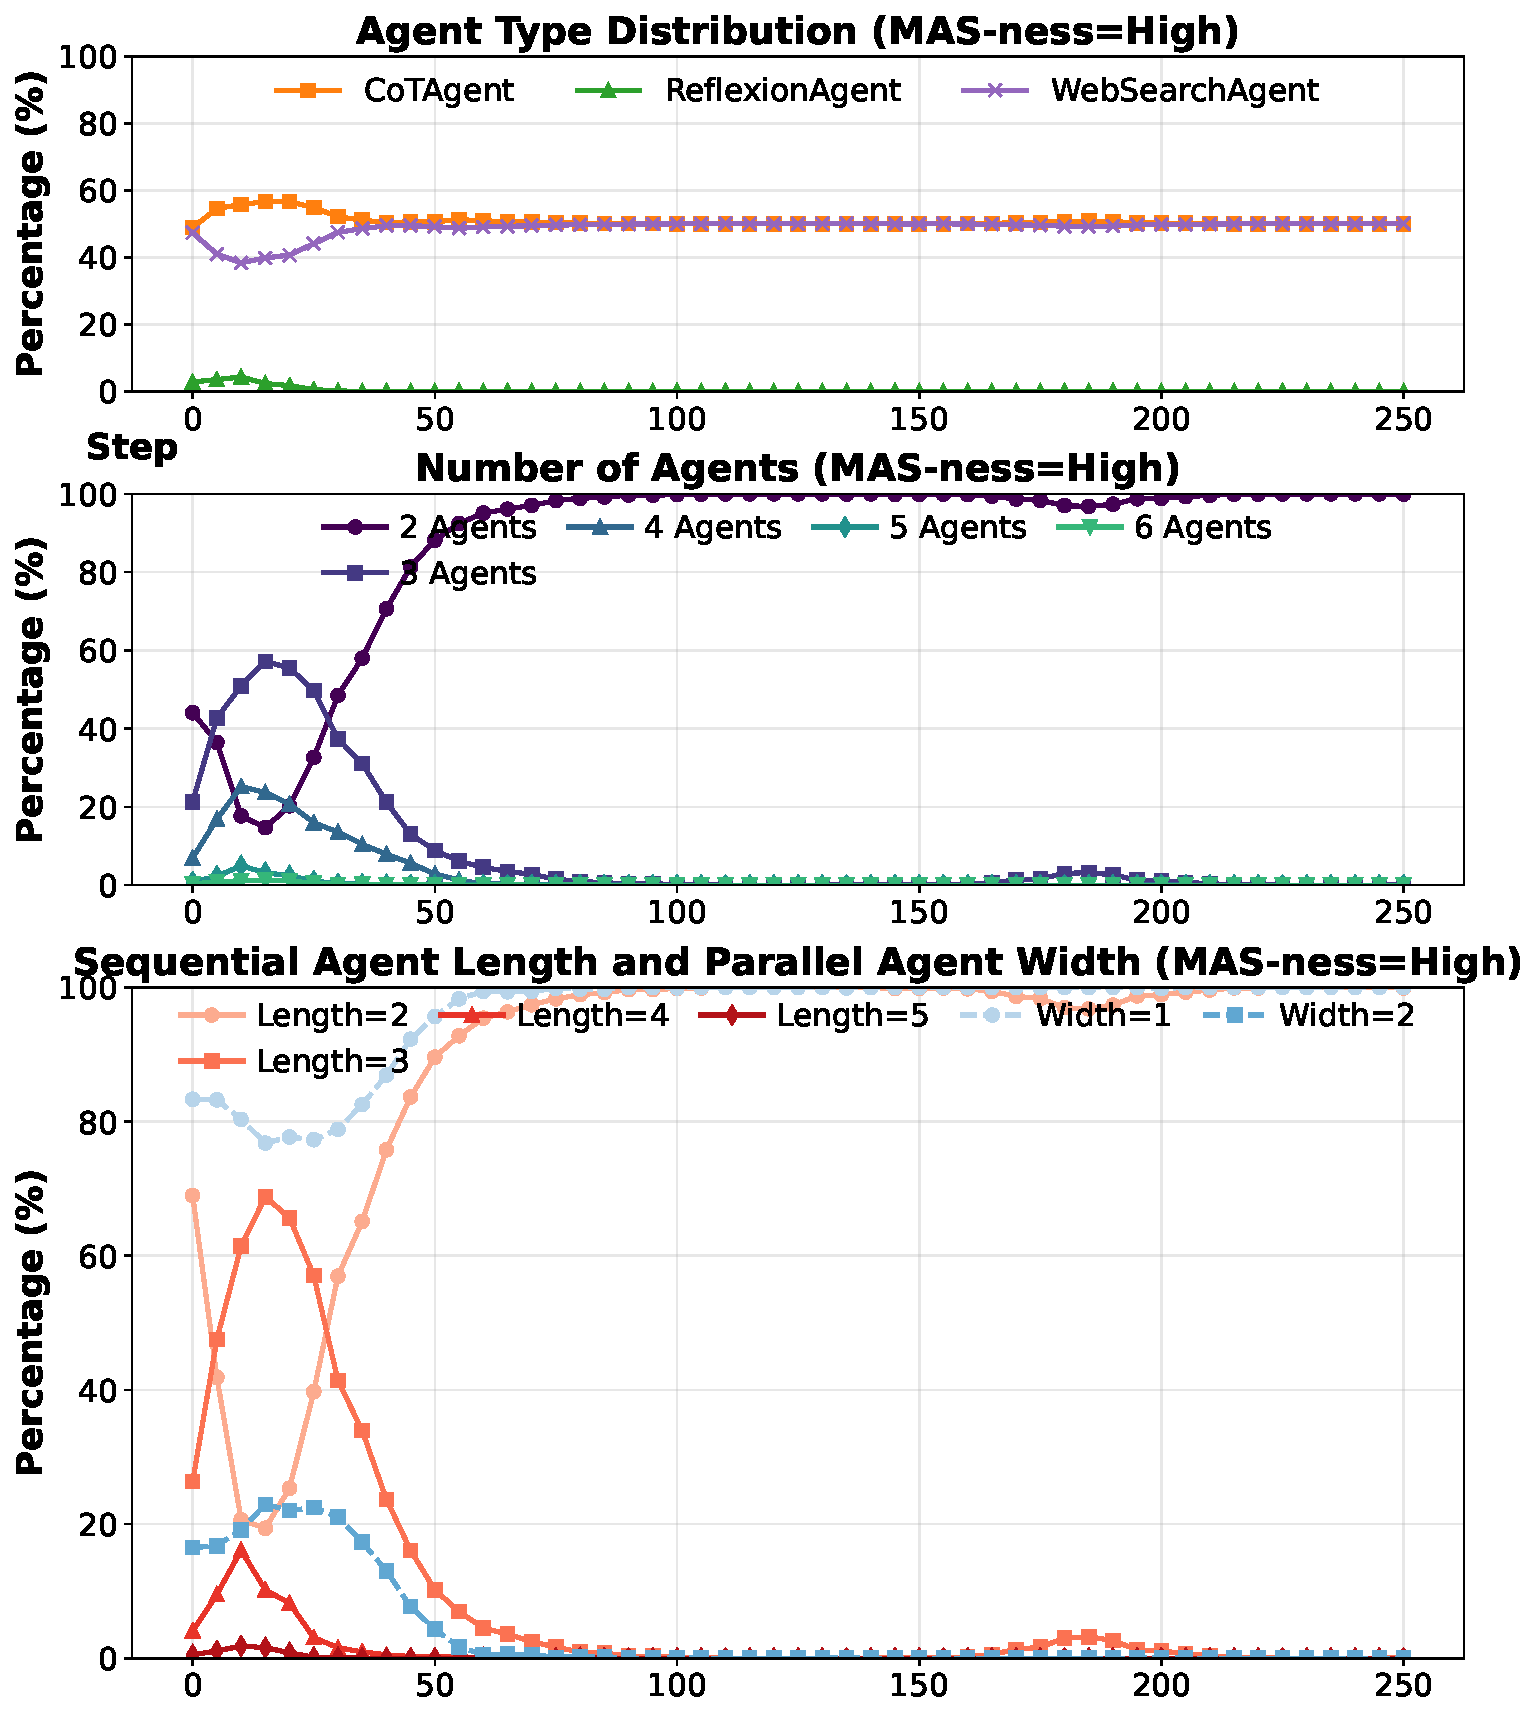
\includegraphics[width=0.5\columnwidth]{figs/7b_120b_hotpotqa_high.pdf}
% \vspace{-\baselineskip}
\captionof{figure}{\small Statistics of agents for \masness as high (HotpotQA).}
\label{fig:7b_120b_hotpotqa_high}
\end{figure*}

\begin{center}
% \vspace{-2\baselineskip}
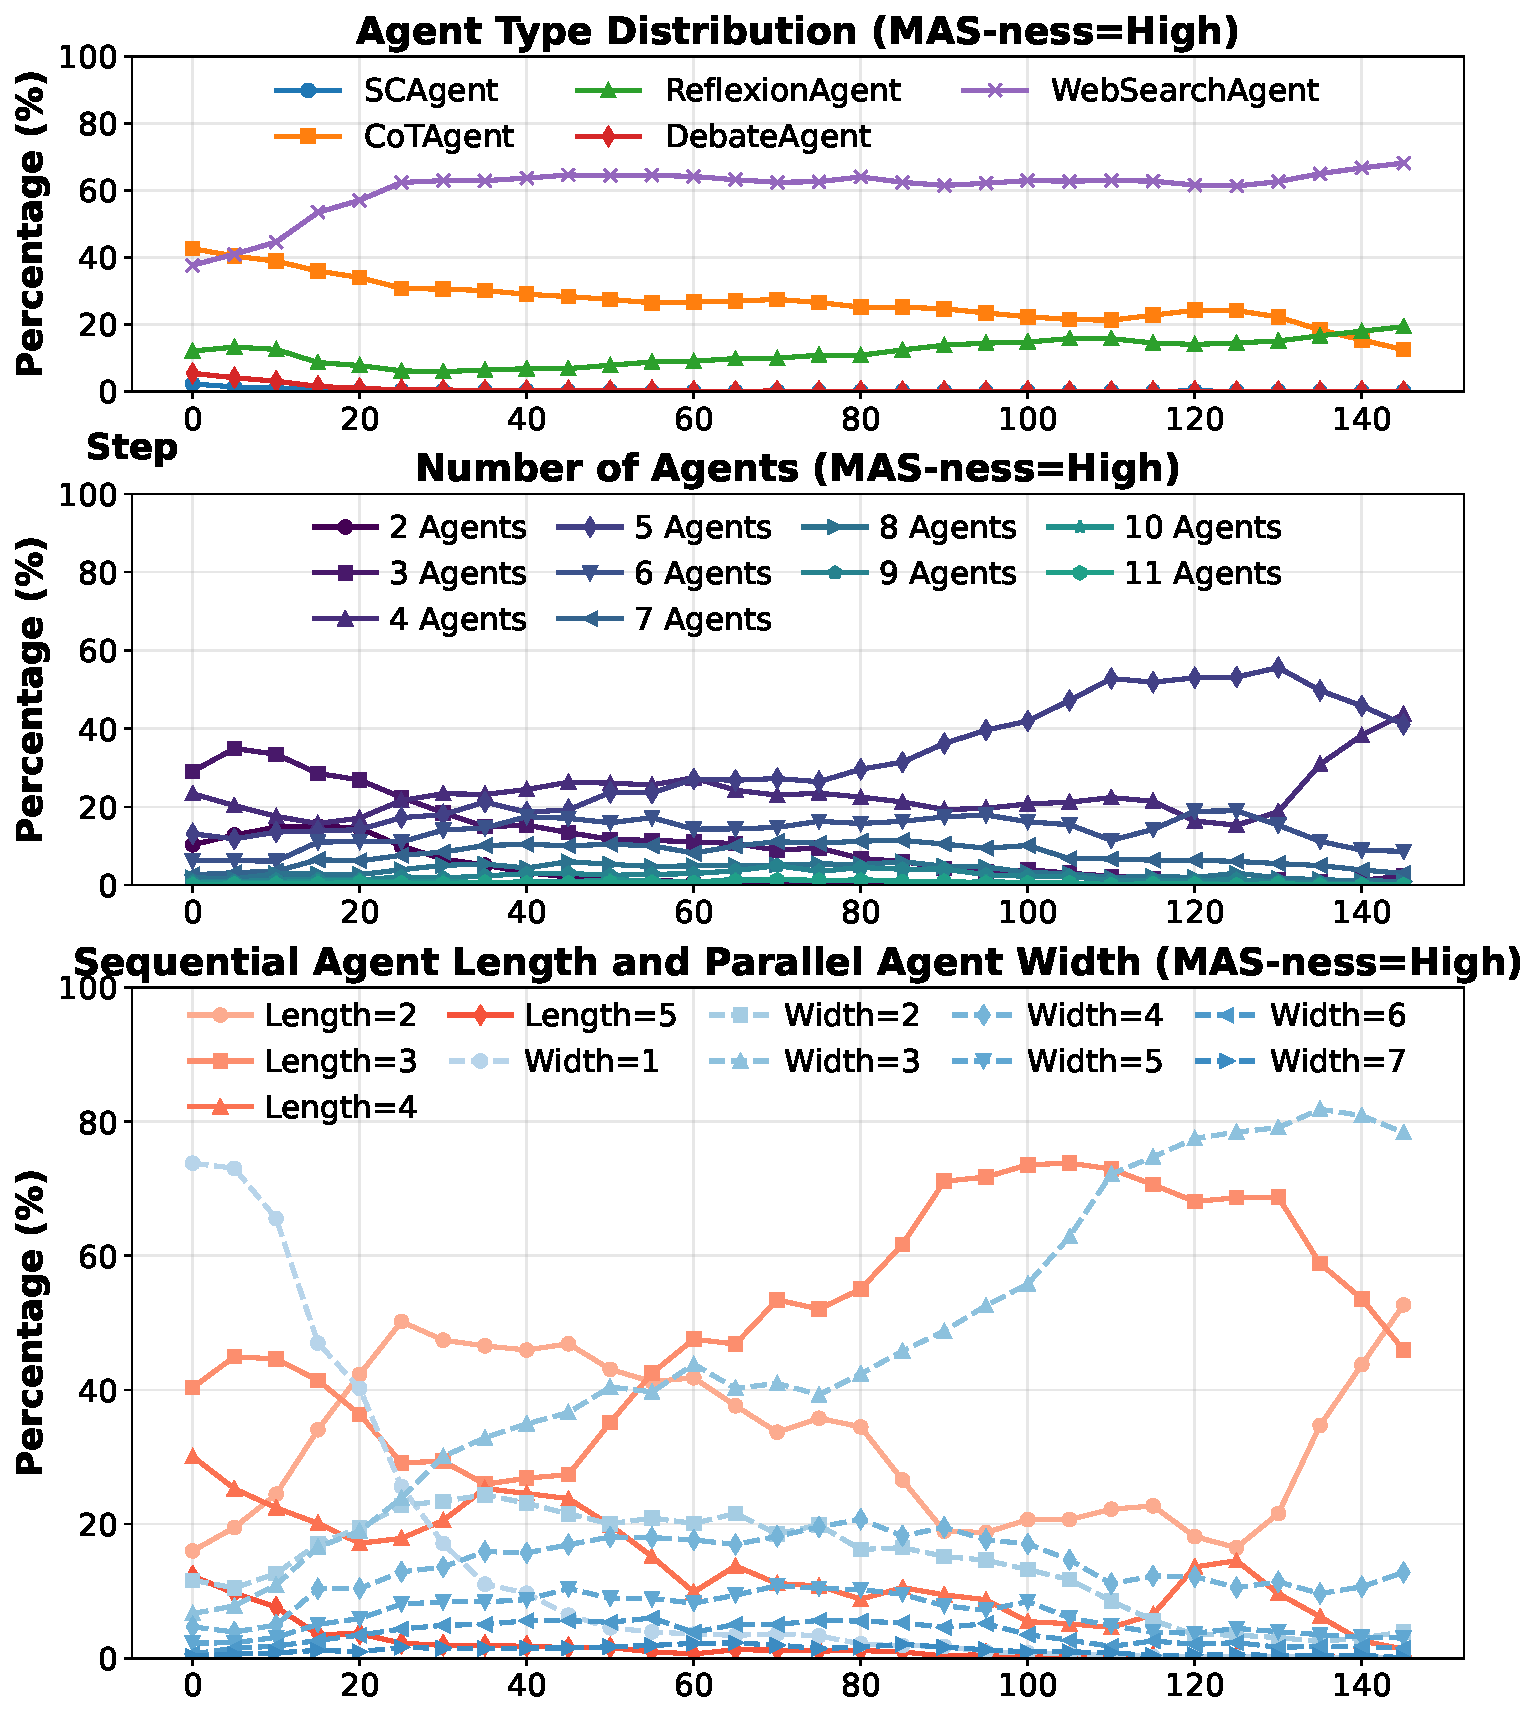
\includegraphics[width=0.5\columnwidth]{figs/7b_120b_browse_comp_plus_high.pdf}
\vspace{-0.5\baselineskip}
\captionof{figure}{\small Statistics of agents for high \masness (BrowseComp+).}
\label{fig:7b_120b_browse_comp_plus_high}
\end{center}

% \zixuan{the others are more like generalization, no tracking during training}


\subsection{Benchmarks vs. Generated MAS}
\label{ap:benchmark_generated_mas}

Beyond the results reported in \cref{sec:experiemnt}, We show the statistics of HotpotQA in \cref{fig:7b_120b_hotpotqa_high}. 
% \textbf{MAS patterns.}
% For AIME24, AIME25, and GPQA, the orchestrator effectively selects the best-performing sub-agent, which is typically the DebateAgent. This suggests that, for reasoning-intensive tasks with limited external information needs, selecting a strong reasoning sub-agent is sufficient.
For HotpotQA, the orchestrator often decides to use only a single \texttt{SearchAgent} (together with a final \texttt{CoTAgent}, for a total of 2 agents), even though the question may allow parallel searches. This suggests that the questions are relatively simple and that one search step is sufficient to solve them. 

Together with the AIME results in Figures \ref{fig:7b_120b_aime24_low} and the BrowseComp+ results in \ref{fig:7b_120b_browse_comp_plus_high}, these observations show that \ourframework can dynamically adapt to a given task by proposing MAS designs that align with the underlying sub-task structure and by delegating execution to the most effective agent configurations. We note that the generated MAS designs do not necessarily perfectly match the underlying task structure (for example, in HotpotQA), due to diverse underlying LLM capabilities, which highlights an advantage over manually designed orchestration strategies.

% We note that this is expected as the orchestrator optimizes only for performance and does not explicitly consider cost or efficiency.

% For BrowseComp+, the orchestrator generates substantially more search agents. The typical pattern first retrieves all potentially required information through multiple search agents and then introduces an organization or aggregation agent to combine the retrieved results. This behavior is intuitive under a single-step reinforcement learning strategy, where collecting comprehensive evidence before aggregation can improve final-answer correctness.



% MAS Pattern: For AIME24, AIME25 and GPQA, orchestrator effectively select the good eprformaining sub-agent (typically DebateAgent). For HotpotQA, orchestrator decided to use only one search agent, while the question may have parallel searches. This indicates the question is relatively simple and one search is good enough (also our orchestrator only considers performance, not cost or efficiency). For BrowseComp+, much more search agents are createad. It typically first searches for all potential required information, and have an organizarion agent to aggregate all the searched results. (this makes intuitively sense for a single-step RL stategy)

% \zixuan{TODO Appendix: add more examples/statistics, e.g, how the 5 agents looks like, why they are good... so that we can discuss more here}


\subsection{Cost Comparison}
\label{ap:cost_breakdown}



In \cref{fig:parato_front}, we illustrate the cost–performance trade-off. In \cref{tab:cost_breakdown}, we report the corresponding detailed inference costs on AIME24 and GPQA. Holistic orchestration is expected to be more efficient than sequential orchestration systems, and even more so compared to inference-time orchestration methods. Consistent with this intuition, \ourframework achieves more than \textbf{10$\times$} efficiency in terms of the number of LLM calls, the number of tokens (including both prompt and completion tokens), and overall cost (based on Together AI pricing at the time of writing). We also observe substantially faster wall-time performance. We note that wall-time reflects not only the algorithmic design but also implementation details, where we apply extensive optimization (e.g. asynchronous sub-agent execution) and will release the full codebase to the community.

% We note that in AIME24 and GPQA, which, as mentioned in \cref{sec:experiemnt}, mainly has the seqeuntail natural, SAS or simple standalone sub-agent can outperformes other automatic MAS design system as they are not in the regime of the edge of the sub-agent cometenece

% \zixuan{TODO: description: walltime is probably not very informative as it relates to implementaiton, async, etc., our implementaion optimize quite a bit on this.}


\begin{table}[h]
\centering
\small
\setlength{\tabcolsep}{6pt}
\renewcommand{\arraystretch}{1.15}
\begin{tabular}{lcccccccc}
\toprule
& \multicolumn{4}{c}{\textbf{AIME24}} & \multicolumn{4}{c}{\textbf{GPQA}} \\
\cmidrule(lr){2-5} \cmidrule(lr){6-9}
\textbf{Method}
& \textbf{Calls}
& \textbf{Tokens (M)}
& \textbf{Cost (\$)}
& \textbf{Time (ks)}
& \textbf{Calls}
& \textbf{Tokens (M)}
& \textbf{Cost (\$)}
& \textbf{Time (ks)} \\
\midrule
CoTAgent
& 30 & 0.05 & 0.03 & 0.38
& 198 & 0.16 & 0.06 & 1.18 \\
SCAgent
& 156 & 0.25 & 0.13 & 1.88
& 990 & 0.80 & 0.29 & 5.43 \\
DebateAgent
& 332 & 0.37 & 0.13 & 2.29
& 2178 & 2.04 & 0.55 & 7.65 \\
ReflexionAgent
& 112 & 0.14 & 0.06 & 0.67
& 518 & 0.44 & 0.13 & 2.50 \\
\midrule
MaAS
& 501 & 1.28 & 0.62 & 6.96
& 2936 & 7.52 & 3.11 & 39.52 \\
AFlow
& 1288 & 3.47 & 1.46 & 19.28
& 7404 & 12.38 & 4.52 & 56.94 \\
\midrule
MAS-GPT
& 228 & 0.74 & 0.37 & 5.47
& 1516 & 3.90 & 1.76 & 29.56 \\
ToolOrchestra
& 1319 & 3.77 & 1.76 & 31.35
& 7829 & 15.38 & 5.79 & 92.47 \\
\midrule
\textbf{\ourframework}
& \textbf{51} & \textbf{0.03} & \textbf{0.01} & \textbf{0.50}
& \textbf{261} & \textbf{0.22} & \textbf{0.07} & \textbf{0.46} \\
\bottomrule
\end{tabular}
\caption{Inference-time statistics on AIME24 and GPQA. Token counts are in millions (M) and wall time in thousands of seconds (ks).}
\label{tab:cost_breakdown}
\end{table}
